

\newcommand\DELTA{0.5}
\begin{figure}[!t]
\centering
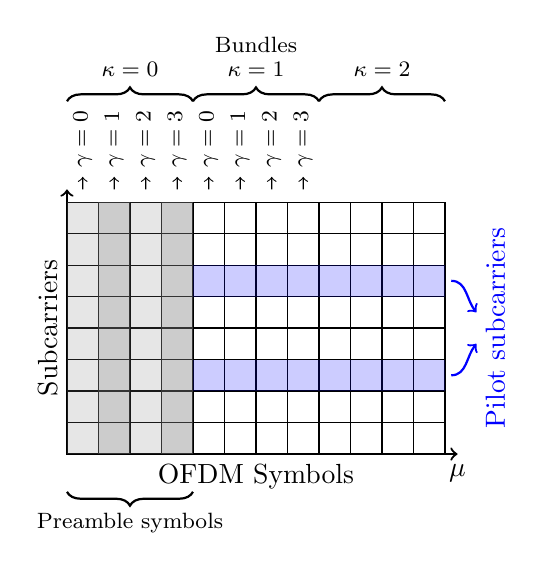
\begin{tikzpicture}[scale=0.8]
% Draw axes
    \draw [<->,thick] (0,4.2) node (yaxis) [left] {}
        |- (6.2,0) node (xaxis) [below] {$\mu$};
%    \node[left] at (0,5-\DELTA/2) {\footnotesize $m=0$};    
%    \node[left, text centered] at (0,\DELTA/2) {\footnotesize $m=N_\text{c}-1$};    
%    \node[below] at (\DELTA/2,0 ) {\footnotesize $\mu = 0$}; 
    \node[left, anchor=south, rotate=90] at (0,2.0) {Subcarriers};
    \node[below] at (3,0) {OFDM Symbols};
% Draw grid
	\draw[step=\DELTA,black,thin,xshift=0cm,yshift=0cm] (0,0) grid (6,4);
%	\draw[step=\DELTA,black,thin, dashed,xshift=0cm,yshift=0cm] (3,0) grid (3.9,4);
% Draw colors
	\draw[draw=none, fill=gray, opacity=0.2] (0,0) rectangle ++(\DELTA, 4);
	\draw[draw=none, fill=gray, opacity=0.4] (\DELTA,0) rectangle ++(\DELTA, 4);
	\draw[draw=none, fill=gray, opacity=0.2] (2*\DELTA,0) rectangle ++(\DELTA, 4);
	\draw[draw=none, fill=gray, opacity=0.4] (3*\DELTA,0) rectangle ++(\DELTA, 4);
%	\draw[draw=none, fill=blue, opacity=0.2] (4*\DELTA,7*\DELTA) rectangle ++(2,\DELTA);


%% channel estimates
%	% nodes
%\node (h0) at (0.25, 5.7) {\footnotesize $\veh{h}_0$};
%\node (h1) at (0.75, 5.4) {\footnotesize $\veh{h}_1$};
%\node (h2) at (1.25, 5.1) {\footnotesize $\veh{h}_2$};
%\node (h3) at (1.75, 4.8) {\footnotesize $\veh{h}_3$};

%% arrows
%  \draw[->, to path={-| (\tikztotarget)}]
%  (0.25,4.2) -- (h0);
%  \draw[->, to path={-| (\tikztotarget)}]
%  (0.75,4.2) -- (h1);
%  \draw[->, to path={-| (\tikztotarget)}]
%  (1.25,4.2) -- (h2);
%  \draw[->, to path={-| (\tikztotarget)}]
%  (1.75,4.2) -- (h3);
  
% Pilots
\draw[draw=none, fill=blue, opacity=0.2] (2,1) rectangle ++(4,\DELTA);
\draw[draw=none, fill=blue, opacity=0.2] (2,2.5) rectangle ++(4,\DELTA);
\draw [->,blue, thick] (6.1, 2.75) to [out=0,in=130] (6.5, 2.25);
\draw [->,blue, thick] (6.1, 1.25) to [out=0,in=-130] (6.5, 1.75);
\node[right, anchor=center, rotate=90, color = blue] at (6.8, 2.0) {Pilot subcarriers};

%% Pilot tone
%	\node (pilot) at (3.25,5.0) {\footnotesize \color{blue}Reference tone\color{black}};
%  \draw[->, to path={-| (\tikztotarget)}, blue]
%  (3.25,3.75) -- (pilot);

% slow-time

% Draw preambles
\draw[decorate,decoration={brace,amplitude=5pt}, thick]  (0,5.6) -- (2,5.6);
\node (pr0) at (1, 6.1) {\footnotesize $\kappa = 0$};
\draw[decorate,decoration={brace,amplitude=5pt}, thick]  (2,5.6) -- (4,5.6);
\node (s0) at (3, 6.1) {\footnotesize $\kappa = 1$};
\draw[decorate,decoration={brace,amplitude=5pt}, thick]  (4,5.6) -- (6,5.6);
\node (s1) at (5, 6.1) {\footnotesize $\kappa = 2$};

\node[align=center] (cu0) at (3, 6.5) {\footnotesize Bundles};


% gamma symbols
\node[right, rotate=90] (g5) at (0.25, 4.4) {\footnotesize $\gamma = 0$};
\node[right, rotate=90] (g6) at (0.75, 4.4) {\footnotesize $\gamma = 1$};
\node[right, rotate=90] (g7) at (1.25, 4.4) {\footnotesize $\gamma = 2$};
\node[right,  rotate=90] (g8) at (1.75, 4.4) {\footnotesize $\gamma = 3$};


\node[right, rotate=90] (g1) at (2.25, 4.4) {\footnotesize $\gamma = 0$};
\node[right, rotate=90] (g2) at (2.75, 4.4) {\footnotesize $\gamma = 1$};
\node[right, rotate=90] (g3) at (3.25, 4.4) {\footnotesize $\gamma = 2$};
\node[right, rotate=90] (g4) at (3.75, 4.4) {\footnotesize $\gamma = 3$};


\draw[->, to path={-| (\tikztotarget)}]
  (2.25,4.2) -- (g1);
  \draw[->, to path={-| (\tikztotarget)}]
  (2.75,4.2) -- (g2);
  \draw[->, to path={-| (\tikztotarget)}]
  (3.25,4.2) -- (g3);
  \draw[->, to path={-| (\tikztotarget)}]
  (3.75,4.2) -- (g4);
  \draw[->, to path={-| (\tikztotarget)}]
  (0.25,4.2) -- (g5);
  \draw[->, to path={-| (\tikztotarget)}]
  (0.75,4.2) -- (g6);
  \draw[->, to path={-| (\tikztotarget)}]
  (1.25,4.2) -- (g7);
  \draw[->, to path={-| (\tikztotarget)}]
  (1.75,4.2) -- (g8);
 
 \node[right, anchor=center, align=center] at (5.0, 5.0) {$\hdots$};
 
 \draw[decorate,decoration={brace,amplitude=5pt}, thick, anchor=center, rotate=180]  (-2,0.6) -- (0,0.6);
 \node[align=center] (cu0) at (1, -1.1) {\footnotesize Preamble symbols};
  
%\node[right, anchor=center, align=center] at (1.0, 0.7) {$\vdots$};
%\node[right, anchor=center, align=center] at (4.0, 0.7) {$\vdots$};

\end{tikzpicture}
\caption{Exemplary allocation of preamble OFDM symbols and pilot subcarriers in $\m{S}$ for DDM.}
\label{fig:Comm_setup_DDM}
\end{figure}



